\begin{frame}
  \frametitle{Optimising \lstinline{lowPass}}

  \begin{itemize}
  \item Cache optimisation: re-order for-loops
  \item Split into two loops, parallelise with OpenMP
  \item 2000ms $\to$ 100ms
  \end{itemize}

\end{frame}

\begin{frame}
  \frametitle{Optimising \lstinline{lowPass}}
  \begin{center}
          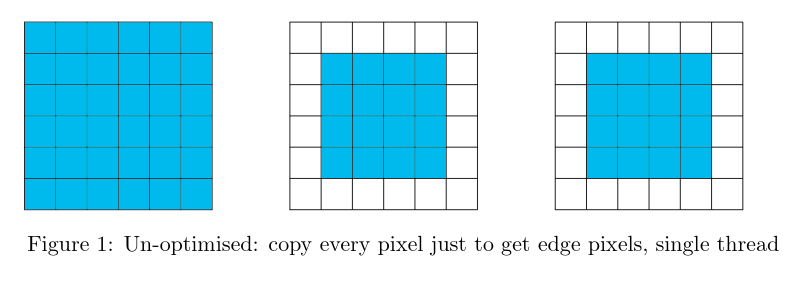
\includegraphics[width=.8\textwidth]{lowPassUnoptimised.png}
  \end{center}
  \begin{center}
            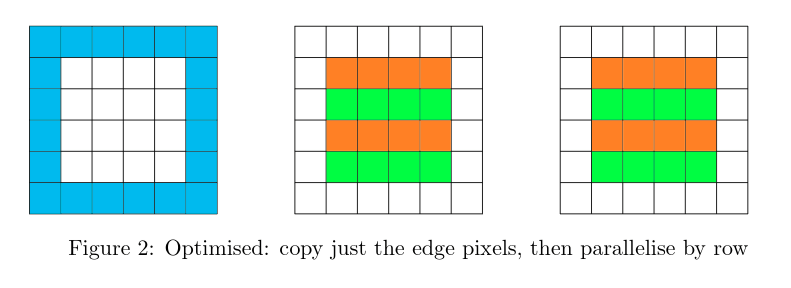
\includegraphics[width=.8\textwidth]{lowPassOptimised.png}
  \end{center}

\end{frame}

% convertRGBtoYCbCr
\begin{frame}
  \frametitle{Optimising \lstinline{convertRGBtoYCbCr}}
  \begin{itemize}
    \item It is better to parallelise with OpenMP than the GPU since the time to transfer data to the GPU is greater than time gained from using the GPU.
    \item 1000ms $\to$ 30ms
  \end{itemize}

  \begin{exampleblock}{}
    \lstinputlisting[basicstyle=\tiny,linerange=84-96]{src/main.cpp}
  \end{exampleblock}

\end{frame}



% loadImage
\begin{frame}
  \frametitle{Optimising \lstinline{loadImage}}
    \begin{itemize}
        \item Unoptimised, loadImage takes 21\% of computation time: good candidate for optimisation.
        \item Using OpenMP, we decreased the absolute time from 860ms to 780ms = 9\% speedup
    \end{itemize}
    \begin{exampleblock}{}
        \lstinputlisting[basicstyle=\tiny,linerange=61-73]{src/main.cpp}
    \end{exampleblock}

\end{frame}

\begin{frame}
  \frametitle{Compilation Flags}
    \begin{itemize}
        \item We used the -O3 compiler optimisation flag. With this flag, the compiler automatically uses SIMD instructions where possible and also does other automatic assembly optimisations like loop unrolling.
        \item We removed the -g debugging flag and added the -march=native and -mtune=native, but these had no visible effect on performance
    \end{itemize}
\end{frame}


%%% Local Variables:
%%% mode: latex
%%% TeX-master: "presentation"
%%% End:
